\documentclass[norsk,a4paper,12pt]{article}
% if you want a single-column, remove reprint

% allows special characters (including æøå)
\usepackage[utf8]{inputenc}
\usepackage [norsk]{babel} %if you write norwegian
%\usepackage[english]{babel}  %if you write english


\usepackage{physics,amssymb}  % mathematical symbols (physics imports amsmath)
\usepackage{graphicx}         % include graphics such as plots
\usepackage{xcolor}           % set colors
\usepackage{hyperref}         % automagic cross-referencing (this is GODLIKE)
\usepackage{tikz}             % draw figures manually
\usepackage{listings}         % display code
\usepackage{subfigure}        % imports a lot of cool and useful figure commands
\usepackage{float}			  % force placement of tables and figures
\usepackage{amsmath}
\usepackage{minted} %code

\hypersetup{ % this is just my personal choice, feel free to change things
	colorlinks,
	linkcolor={red!50!black},
	citecolor={blue!50!black},
	urlcolor={blue!80!black}}

%% Defines the style of the programming listing
%% This is actually my personal template, go ahead and change stuff if you want
\lstset{ %
	inputpath=,
	backgroundcolor=\color{white!88!black},
	basicstyle={\ttfamily\scriptsize},
	commentstyle=\color{magenta},
	language=Python,
	morekeywords={True,False},
	tabsize=4,
	stringstyle=\color{green!55!black},
	frame=single,
	keywordstyle=\color{blue},
	showstringspaces=false,
	columns=fullflexible,
	keepspaces=true}

\title{FYS3110 - Oblig 1 - Karl Henrik Fredly}

\begin{document}
	
	\maketitle
	
	\section*{Problem 1.6(H)}
	
	\subsection*{a)}
	\begin{equation}
	\begin{aligned}
	\int_{-\infty}^{\infty}\delta_\epsilon(x)dx &=
	\int_{-\infty}^{\infty}\frac{1}{\pi} \frac{\epsilon}{\epsilon^2 + x^2}dx =
	\frac{1}{\pi} \frac{\epsilon}{\epsilon^2}\int_{-\infty}^{\infty} \frac{1}{1 + (\frac{x}{\epsilon})^2}dx
	\end{aligned}
	\end{equation}
	setter $u = \frac{x}{\epsilon}$. Finner $\frac{du}{dx} = \frac{1}{\epsilon} \Rightarrow dx = \epsilon du$.
	\begin{equation}
	\begin{aligned}
	\int_{-\infty}^{\infty}\delta_\epsilon(x)dx &=
	\frac{1}{\pi} \frac{\epsilon^2}{\epsilon^2}\int_{-\infty}^{\infty} \frac{1}{1 + u^2}du \\
	&= \frac{1}{\pi} [arctan(u)]_{-\infty}^{\infty} = \frac{1}{\pi} [\frac{\pi}{2} + \frac{\pi}{2}] = 1
	\end{aligned}
	\end{equation}
	
	\subsection*{b)}
	\begin{equation}
	\begin{aligned}
	\delta_\frac{\epsilon}{k}(x) &= \frac{1}{\pi} \frac{\frac{\epsilon}{k}}{(\frac{\epsilon}{k})^2 + x^2} \\
	&= \frac{1}{\pi} \frac{\frac{\epsilon}{k}}{(\frac{\epsilon}{k})^2 + x^2} \frac{k^2}{k^2} \\
	&= k\frac{1}{\pi} \frac{\epsilon}{\epsilon^2 + k^2x^2} \\
	&= k\frac{1}{\pi} \frac{\epsilon}{\epsilon^2 + (kx)^2} \\
	&= k \delta_\epsilon(kx)
	\end{aligned}
	\end{equation}
	
	\subsection*{c)}
	\begin{minted}[mathescape, linenos]{python}
		import numpy as np
		import matplotlib.pyplot as plt
		
		def delta(eps, x):
			return 1/np.pi * eps / (eps**2 + x**2)
		
		n = 1000
		x = np.linspace(-1, 1, n)
		
		plt.figure(figsize = (8, 6))
		for eps in [0.01, 0.1, 1]:
			plt.plot(x, delta(eps, x), label=eps)
		plt.legend()
		plt.show()
	\end{minted}

	\begin{figure}[H]
		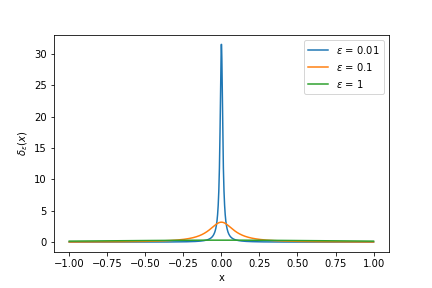
\includegraphics[width=150mm]{../16bfig.PNG}
	\end{figure}
	
	\subsection*{d)}
	Man kan få en tabell med argumenter og verdier for $\delta_{0.1}$ fra en tabell med argumenter og verdier for $\delta_{1}$ ved å skalere argumentene og funksjonsverdiene med 10. Siden
	
	\begin{equation}
	\begin{aligned}
	\delta_\frac{\epsilon}{k}(x) &= k \delta_\epsilon(kx) \Rightarrow \delta_{\frac{1}{10}}(x) = 10 \delta_1(10x)
	\end{aligned}
	\end{equation}
	
	f.eks: $\delta_{\frac{1}{10}}(0.5) = 10 \delta_1(5)$.
	
	\section*{Problem 1.7(H)}
	
	\begin{equation}
	\begin{aligned}
	\hat{P_1}\ket{A} = \ket{b_1} \braket{b_1}{A} = \ket{b_1} \Sigma_{i=1}^{N} a_i \braket{b_1}{b_i} = a_1 \ket{b_1}
	\end{aligned}
	\end{equation}
	siden $\braket{b_1}{b_i} = 1$ for i = 1 og 0 ellers.
	
	\begin{equation}
	\begin{aligned}
	\hat{P_1}\hat{P_1}\ket{A} = \ket{b_1} \braket{b_1}{b_1} \braket{b_1}{A} = \ket{b_1} \Sigma_{i=1}^{N} a_i \braket{b_1}{b_i} = a_1 \ket{b_1}
	\end{aligned}
	\end{equation}
	siden $\braket{b_1}{b_1} = 1$.
	
	$\hat{P_1}$ kalles en projeksjonsoperator fordi den returnerer projeksjonen av en vektor langs vektoren $\ket{b_1}$. Det gjør da ingen forskjell om man benytter den flere ganger på samme vektor.
	
	\section*{Problem 1.8(X)}
	En kvantetilstand er et matematisk uttrykk som gir en fullstendig beskrivelse av et fysisk system. En kvantetilstand blir representert ved en vektor, og den beskriver ofte sannsynlighetsfordelingen til ulike observable verdier til systemet. En klassisk tilstand blir i motsetning beskrevet med konkrete verdier uten usikkerheter.
	
\end{document}